\FloatBarrier
\subsection{Audio Pipelines}\label{subsec:audio_pipelines}

\begin{figure}[H]
    \centering
    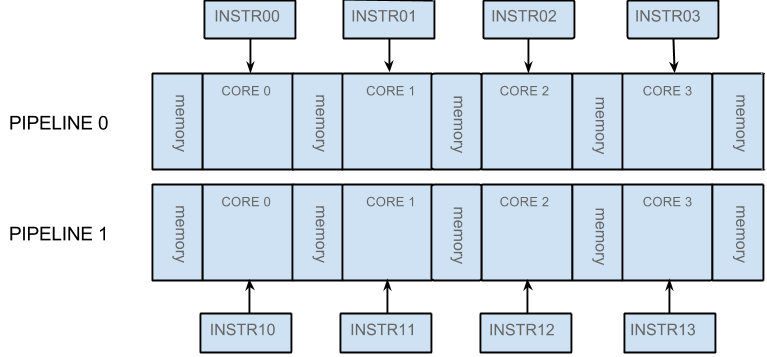
\includegraphics[height=150px]{figures/fpga/system_components_general_pipeline_without_programs.png}
    \caption{Audio Pipeline Architecture}
    \label{fig:pipeline_architecture}
\end{figure}

The FPGA design consists of several audio processing pipelines, as illustrated in
figure \ref{fig:pipeline_architecture}. These contain several processing cores
separated by data buffers. Each audio processing pipeline processes one channel
of sound data.

